\chapter{From Work Stealing to Reactive Load Balancing}
\label{ch:wstoreactlb}
\index{FromWS2ReactLB!From Work Stealing to Reactive Load Balancing}
\chaptertoc
\noindent

Based on the overview in Chapter \ref{ch:Introduction}, Chapter \ref{ch:wstoreactlb} provides in more detail terminologies, task-based programming models and runtimes, applications and state-of-the-art related to dynamic load balancing in distributed memory systems. The content of Chapter \ref{ch:wstoreactlb} is summarized in Figure \ref{fig:chapter_two_overview} as an inverted pyramid. First, the top view of parallel computing is shown in Section \ref{sec:preliminaries} and we describe in more detail the concepts as well as terminologies associated with the architecture of distributed memory systems. Second, we go in-depth on how programming models are designed for shared and distributed memory systems in Section \ref{sec:taskbased_prog_models}. Hereby, task-based parallel programming models are emphasized as an instrument to research dynamic load balancing. Following that, task-based parallel runtimes and applications are addressed as the objects introduced in Section \ref{sec:taskbased_runtimes_apps}. Finally, the related work from work stealing to reactive load balancing is analyzed in Section \ref{sec:relatedwork}.

\begin{figure}[h]
  \centering
  \includegraphics[scale=0.75]{./pictures/preliminaries/preli_parallelcomp_overview.pdf}
	\caption{The overview of Chapter \ref{ch:wstoreactlb}}
	\label{fig:chapter_two_overview}
\end{figure}

\section{Preliminaries}
\label{sec:preliminaries}
\index{FromWS2ReactLB!Preliminaries}

The majority of applications are written as serial or sequential computations. However, suppose our applications have complex computations and are able to be broken into smaller tasks running simultaneously. In that case, the concept of parallel computing can be applied to reduce overall execution time. Parallel computing denotes the use of multiple computing resources to execute a computational problem simultaneously. This leads to the motivation of parallelism in both software and hardware. Software refers to parallel applications, programming models, or support libraries. Hardware refers to parallel computing technology, such as multicore architectures or compute clusters.\\

\begin{figure}[t]
  \centering
  \includegraphics[scale=0.425]{./pictures/preliminaries/preli_parallel_computing_and_taxonomy.pdf}
	\caption{A generic view of parallel computing \cite{hpcllnl2023parcomp}.}
	\label{fig:preli_parallel_computing_and_taxonomy}
\end{figure}

\noindent \textbf{Parallelism}: can happen in different forms, e.g., bit-level parallelism, instruction-level parallelism, data parallelism, and task parallelism \cite{kumar1994intro} \cite{hpcllnl2023parcomp}. Simply put, we assume that a program includes a series of instructions. Sequentially, the program executes one instruction after another, where only one processor is used, and one instruction is executed at once. In parallel, the program can be split into smaller parts running on different processors, where each part now includes a subset of instructions. At the same time, the instructions of different parts can be scheduled to run on different processors. Figure \ref{fig:preli_parallel_computing_and_taxonomy} (A) illustrates an example of parallel computing with four processors. From left to right, we can see the problem divided into four parts, shown as $Part\ 1$, $Part\ 2$, $Part\ 3$, and $Part\ 4$. Each part includes instructions that are scheduled for executing simultaneously on four processors (indexed from $Processor\ 0$ to $Processor\ 3$).\\

Regarding classification, Flynn's taxonomy \cite{kumar1994intro} is widely used. There are four classes shown in Figure \ref{fig:preli_parallel_computing_and_taxonomy} (B), including SISD, SIMD, MISD, and MIMD. Each class is depicted next to its corresponding acronym. The main distinction is based on \textbf{Instruction Stream} and \textbf{Data Stream}, corresponding to the view of von Neumann Computer Architecture \cite{eigenmann1999vonneumanarch}. In detail, each class is characterized as follows.

\begin{itemize}
	\item SISD: Single Instruction Single Data (illustrated in Figure \ref{fig:preli_parallel_computing_and_taxonomy} (B) under the acronym, SISD). Only one instruction is performed, and one data item is manipulated at a time. One arrow stands for an instruction loaded from the instruction pool, and another stands for data manipulation.
	
	\item SIMD: Single Instruction Multiple Data (illustrated in Figure \ref{fig:preli_parallel_computing_and_taxonomy} (B) under the acronym, SIMD). This class of parallel computing has multiple processors, where each processor runs the same instruction on its own data.
	
	\item MISD: Multiple Instruction Single Data (illustrated in Figure \ref{fig:preli_parallel_computing_and_taxonomy} (B) next to the acronym, MISD).
	
	\item MIMD: Multiple Instruction Multiple Data (illustrated in Figure \ref{fig:preli_parallel_computing_and_taxonomy} (B) next to the acronym, MIMD), showing that multiple processors execute multiple instructions and operate multiple data items simultaneously.
\end{itemize}

Expanding from MIMD, some researches divide it into the programming models called Single Program Multiple Data streams (SPMD) \cite{daerma2001spmdmodel} and Multiple Programs Multiple Data streams (MPMD) \cite{fzj2023mpmdmodel}.\\

\begin{figure}[t]
  \centering
  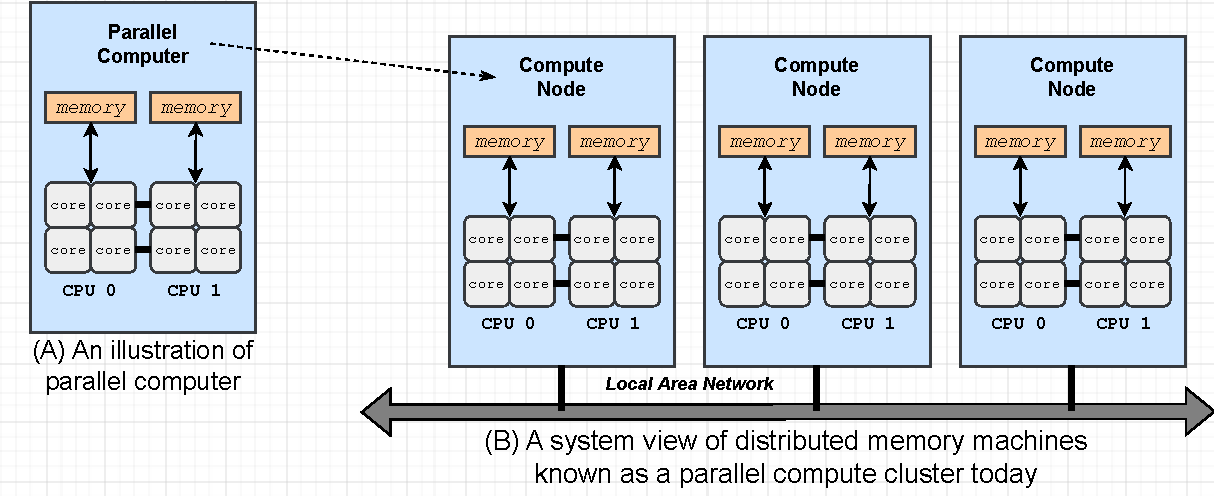
\includegraphics[scale=0.6]{./pictures/preliminaries/preli_parallel_and_distributed_memory_machines.pdf}
	\caption{An example of parallel computers and distributed memory systems know as a parallel compute cluster.}
	\label{fig:preli_parallel_computer_and_cluster}
\end{figure}

\noindent \textbf{Parallel computers:} refers to a computer or a machine with more than one processor (CPU). Sometimes, people imply a CPU as a CPU socket, the physical interface on a motherboard where a CPU is located. In modern computing architectures, a CPU contains multiple cores called single processing units, and each core can execute instructions independently. Each CPU can have its individual memory, where the total memory in a parallel computer is the sum of all individual memories. Figure \ref{fig:preli_parallel_computer_and_cluster} (A) reveals an example of a parallel computer with two CPUs, each with its own memory and containing four cores.\\

Memory access in parallel computers is a complex topic. We can also use the types of memory access to characterize the type of parallel computers. There are mainly two types, shared memory and distributed memory. Shared memory can be noted with all processors accessing the same memory, or a so-called shared address space. Distributed memory can be seen that each CPU has a memory and each refers to a variable on its own memory.\\

From the view of hardware manufactures, the memory architectures of parallel computers are known as
\begin{itemize}
	\item Uniform Memory Access (UMA): all memory locations are accessible to all processors. The access time can be assumed to be identical. A limitation of UMA is the maximum number of processors that can be difficult to expand.
	
	\item Non-Uniform Memory Access (NUMA): each process has a separate memory. This memory architecture can deal with the limit of UMA but leads to a situation where a processor or the cores of a processor access its own memory (local memory) fast and access the other processors' memory (remote memory) slower. Distributed memory implies that a processor cannot directly see another processor's memory. From the programmer's view, there can be a reference to physically and logically distributed memory, which means whether memory is distributed or just appears distributed \cite{victor2010introhpc}. NUMA can be seen as logically and physically distributed, although the distributed nature of NUMA is not apparent to the programmer. Today, most modern computers are made with multicore processors and NUMA architectures.
\end{itemize}

In general, the goal of using parallel computing is to get higher computation performance and access more memory. However, as scientific problems scale up, the complexity of solving them can take a long time to execute on a single computer. Therefore, the idea of parallel compute clusters was built and widely used.\\

\noindent \textbf{Parallel compute clusters:} refers to the architecture used in most supercomputers today. Parallel compute clusters are examples of distributed memory systems. A cluster consists of many computers; in particular, we imply many parallel computers, as explained above. The computers in a cluster are so-called compute nodes. Figure \ref{fig:preli_parallel_computer_and_cluster} (B) demonstrates a parallel compute cluster. All compute nodes can operate as a unified system. Each node connects to another via a local area network (the so-called interconnection network) \cite{baker1999cluster}. The exchange of data or messages between different processors across different nodes is physically distributed memory, where communication overhead might affect the performance of parallel applications. In this thesis, distributed memory indicates the view of memory access in parallel compute clusters. \\

\noindent \textbf{Terminologies}: summarize and emphasize several terminologies based on the explanation above. The following might repeat some notations as well as terms used throughout the thesis.

\begin{itemize}
	\item Cluster: denotes a parallel compute cluster, and is also called an HPC cluster, HPC system, or supercomputer.
	
	\item Node: indicates a compute node in a cluster. Inside a compute node, we have
	\begin{itemize}
		\item Processor or CPU: indicates central processing unit. In computer hardware, a CPU is placed in a CPU socket, which contains mechanical components providing mechanical and electrical connections between a microprocessor and a printed circuit board (PCB). Sometimes, a mentioned CPU socket can also be understood as referring to a CPU.
		\item Core: is single processing unit in a processor. There can be multiple cores inside a processor. Different cores in a node can belong to the same processor or different processors. At the operating system (OS) level, there are
		\begin{itemize}
			\item Process: is an instance of a program. When a process is created and executed, it is defined with its own resources, e.g., memory, file descriptors.
			\item Thread: is an entity within a process. A process can spawn multiple threads inside. While processes are isolated, threads share memory and address space.
		\end{itemize}

		Depending on context switching and mapping algorithm, processes or threads can be mapped dynamically to cores. For performance purposes, a process or thread is often pinned to a specific core in HPC, reducing context switching time. Furthermore, a technology introduced by manufacturer Intel is hyperthreading (Hyper-Threading Technology as HTT or HT) that a single core can run multiple threads. In this case, we call them logical cores in a physical core.
		
	\item Memory: this thesis refers to NUMA architecture in a node (NUMA domain). Each CPU has an individual memory, often called a NUMA node. However, we avoid using NUMA node to ensure no conflict with ``node'' in compute node. We consider the view of memory access in a single node as shared memory. Therefore, it is important to note that
		\begin{itemize}
			\item Shared memory: indicates memory access in a single node.
			\item Distributed memory: indicates memory access across nodes.
		\end{itemize}
	\end{itemize}
	
	\item Communication: implies data or information exchange among processes. These processes can be inside a node or across nodes. To evaluate communication speed, bandwidth is defined as the maximum transmission performance of a network. Generally, bandwidth ($B$) today is measured by megabits, megabytes, or gigabytes per second (Mbps, MBps, or GBps). In HPC networks, communication overhead refers to
	\begin{itemize}
		\item Latency ($\lambda$): the delay time between sending and receiving the header of a message. $\lambda$ can be measured in seconds or milliseconds.
		\item Transmission time or Delay time ($d$): the time for transmitting an entire message between two nodes. Delay ($d$) depends on the size of a message. In the case of no conflict, $d = \lambda + \frac{s}{B}$, where $s$ is the message size. 
	\end{itemize}

\end{itemize}

From the application perspective, users can implement parallel applications using different programming models. The next section introduces general and widespread parallel programming models in common use. Following that, we emphasize our focus on task-based parallel programming models and task-based parallel applications to deal with dynamic load balancing.


% Regarding MPI applications, we might use ranks as an alternative name for processes. Therefore, rank and process can be used interchangeably.
	
%	\item Task: there are different ways to define a task. People may call a task a discrete logical section of computational work. In another context, a task can be a program or a set of instructions executed in sequential or parallel by one or multiple threads/processes. In the thesis's context, we define a parallel program with many tasks.

%	\item Synchronization: denotes the coordination of parallel tasks in real-time. The downsize of synchronization implies waiting for at least one task. Therefore, it can cause a parallel application's wall clock execution time.
%
%	\item Computational Granularity: implies a quantitative or qualitative measure between computation and communication. There are two common terms: \textit{coarse} and \textit{fine}.
%	\begin{itemize}
%		\item Coarse: indicates many computational tasks between communication events.
%		\item Fine: means a small number of computational tasks between communication events.
%	\end{itemize}
%
%	\item Speedup: is a ratio of wallclock execution time between serial execution and parallel execution.
%
%	\item Parallel Overhead: is related to the required execution time, including influence factors such as task start-up time, synchronization, data movement, software overhead, and task termination time.
%
%	\item Scalability: is associated with the ability of a parallel system that can show a proportionate increase in speedup. Several factors, such as hardware, application algorithm, parallel overhead, and application characteristics, can contribute to scalability.

%\textbf{Architectures}: parallel computing systems are mainly designed upon memory models. Almost all machines today revolve around three architectures: shared memory, distributed memory, and hybrid distributed-shared memory.
%\begin{itemize}
%	\item Shared memory machines: is commonly designed with the ability of all processors to access memory like global address space. This architecture has been classified as Uniform Memory Access (UMA) and Non-Uniform Memory Access (NUMA, as mentioned). UMA is  Symmetric Multiprocessor (SMP) with identical processors and equal access time to memory. In contrast, NUMA has a physical link between two or more SMPs. One SMP can access the memory region of another SMP, and they will not have equal access time due to across links.
%	\item Distributed memory machines: often implies a communication overhead via network to link one processor's memory to another. We do not have global address space across all processors because each has its own local memory. Programmers have to define how and when tasks or data are communicated. Importantly, synchronization is essential, and it often belongs to the programmer's responsibility
%	\item Hybrid distributed-shared memory machines: ``hybrid'' refers to the memory model that works on both CPU and graphic processing unit (GPU)/accelerators. There are two main components: shared memory component and distributed memory component. The shared component indicates the connection between CPU and GPU, while the distributed component means the connection between multiple CPU/GPU machines. The current trends show that this computing architecture will be more and more popular in future computing technologies.
%\end{itemize}

%	%---------------------------------
%	\item Distributed memory systems
%	%---------------------------------
%	\begin{itemize}
%		\item Fixed: the number of connections between nodes is fixed. When more processors or nodes are added, they have to share, e.g., Ethernet interconnection.
%		\item Linear: the number of connnections grows linearly when the number of nodes is increased, e.g., mesh-based interconnection.
%		\item Scalable: the number of connections grows as $P\log P$ or even greater, e.g., hypercube interconnection.
%	\end{itemize}
%\end{itemize}

%\input{content/Related-Work}

%\vfill
%\section*{Chapter Summary}
%Chapter~\ref{ch:Motivation} provides the motivation, scopes the problem and derives a requirements' analysis for
%a reference model for \pne management systems for \glspl*{HPC system}.
%Additionally, the related work is presented.
%This presents the problem domain analysis according to the methodical approach of this work (see Sec.~\ref{sec:Intro-Method}).
%
%\begin{figure}[H]%[ht]
%    \centering
%    \resizebox{.98\textwidth}{!}{%
%        \input{pictures/Thesis-Method-Gray/Thesis-Method-Gray2.tikz}
%        }
%        \caption[Method Completion After Chapter 2.]{%
%            Method completion after Chapter 2.}
%            \label{fig:Method-Completion2}
%\end{figure}


% 2.1 Parallel Programming Models
\section{Task-based Parallel Programming Models}
\label{sec:taskbased_prog_models}
\index{FromWS2ReactLB!Parallel Programming Models}
% ---------------------------------
% Example for using \si command
% ---------------------------------
% In the advance from \si{peta\gls*{FLOPS}} to \si{exa\gls*{FLOPS}} performance the issues of \pne present a major hurdle. The associated challenges are identified and tackled by different entities in various ways.

A programming model forms an abstraction layer that connects user applications and parallel computer architectures, leveraging a programming-support library/runtime. Before the advent of task-based parallel programming models, shared and distributed memory models have been used mainly. However, there is no clear boundary of these models. The model design relies on the development of computing and memory architectures, such as multicore, manycore, NUMA architectures. The following introduces conventional models, then details the principle of task-based parallel models.\\

\begin{figure}[t]
  \centering
  \includegraphics[scale=0.485]{./pictures/preliminaries/preli_conventional_parallel_prog_models.pdf}
	\caption{An overview of shared memory and distributed memory programming models along with their hybrid model.}
	\label{fig:preli_conventional_parallel_prog_models}
\end{figure}

\noindent \textbf{Shared Memory Programming Model}: enables processes or threads to share a common address space. In this model, processes or threads can communicate and synchronize by reading/writing directly from/to shared memory locations. The model allows efficient data sharing. Figure \ref{fig:preli_conventional_parallel_prog_models} (A) illustrates a parallel program using shared memory programming with threads. Here, Thread 0, 1, 2 execute the instructions simultaneously, and the data such as array A and array B are shared. Shared memory programming can be characterized by:
\begin{itemize}
	\item Advantage: simple and straightforward to write programs in parallel. Communication between processes/threads is faster and more efficient than other models requiring inter-process communication.
	\item Disadvantage: difficult to manage data locality. There are challenges in dealing with complex synchronization, race conditions. Incorrect management of shared memory locations can lead to bugs. Furthermore, the scalability might be limited in the scope of a single machine.
	\item Implementation: the most common library is POSIX threads (so-called Pthreads) \cite{butenhof1997programming}. Besides that, OpenMP \cite{dagum1998openmp} is an industry-standard library to support shared memory programming, widely used in various operating systems and compilers. 
\end{itemize}

%\item Threads model: denotes parallel programs using threads. A heavy process can spawn multiple ``lightweight'' threads with concurrent execution paths. Besides POSIX standard, there is another popular API named OpenMP , an industry standard that is easy to use with directive-based declaration.
%This might be considered as the simplest parallel programming model, but sharing can raise contention problems such as race conditions, deadlocks. Various mechanisms called locks/semaphores are proposed. The model has some characteristics as follows.
%Besides, as mentioned, several implementations working on distributed memory machines can also work with shared memory, for example, SHMEM \cite{chapman2010introducing}. Therefore, people often refer to shared memory with or without threads.

\noindent \textbf{Distributed Memory Programming Model}: does not have a shared address space. Distributed memory in this thesis points to physically distributed memory systems where compute nodes connect to each other via a network. Note that memory architectures can also be called distributed in a single machine with NUMA architecture. However, it just appears as distributed memory from the programming view. We demonstrate a distributed memory programming example in Figure \ref{fig:preli_conventional_parallel_prog_models} (B), assuming we have two compute nodes, each creates a process to execute parallel application. The only way to exchange information across these nodes is message passing. For example, Process 2 sends a message to Process 1 and vice versa. Distributed programming models can be characterized by:
\begin{itemize}
	\item Advantage: data and information are exchanged explicitly by sending and receiving messages. Programmers can coordinate nodes to execute tasks and share data on large problems. The scalability of this model is well-suited for HPC and large-scale parallel applications.
	\item Disadvantage: communication overhead is challenging in data decomposition and combination. The problem in a distributed memory model is divided into smaller parts, which are distributed over nodes. After execution, their results and required data need to be combined, which may take time and overhead. Load balancing is also a challenge when task distribution is irrelevant to the system performance model.
	\item Implementation: the most popular library is based on the Message Passing Interface (MPI) standard \cite{gropp1996mpich}. MPI supports API and subroutines that users can define data exchange communication explicitly or implicitly. Besides, several libraries that support message passing at higher levels can also be characterized as distributed memory programming models known as Partitioned Global Address Space (PGAS) \cite{dewael2015pgasl}. PGAS provides an abstraction layer for programmers. We may not need to define the communication of data exchange explicitly. In this thesis, we classify the programming models like PGAS as data-parallel programming models.
\end{itemize}

\noindent \textbf{Data Parallel Programming Model}: refers to Partitioned Global Address Space (PGAS) \cite{dewael2015pgasl}. The idea is to achieve a higher level of abstraction from a programmers perspective. Even on shared or distributed memory, it treats address space globally. For example, the global data structure can be split up logically across tasks in distributed memory systems. Data parallel programming can be characterized by:
\begin{itemize}
	\item Advantage: user-friendly from the programming point of view. The model shows considerable benefits on regular data structures like arrays or matrices.
	\item Disadvantage: in some use cases with complicated data structures, this model cannot ensure performance as well as portability, such as data locality references, the distribution of sparse and irregular data objects. These are important issues for evaluating the efficiency of data-parallel programming models.
	\item Implementation: several implementations such as Coarray Fortran \cite{mellor2009new}, UPC \cite{zheng2014upc}, X10 \cite{chrles2005x10}, Chapel \cite{chamberlain2007chapel}.
\end{itemize}

\noindent \textbf{Hybrid Programming Model}: refers to combining more than one programming model. We have mentioned the hybrid model of shared memory and distributed memory programming, such as MPI+X or MPI+OpenMP \cite{rabenseifner2009hybrid} in Chapter \ref{ch:Introduction}. Shared memory programming models such as OpenMP allow users to specify shared memory locations and threads, but the scalability is limited in a single node. Distributed memory programming models such as MPI allow users to specify communication patterns and processes across nodes. A MPI process is denoted as MPI rank. In MPI-based applications, message passing can occur inside a node when we fully create the number of MPI ranks corresponding to the number of cores. Therefore, the hybrid model exploits benefits from both shared memory and distributed memory programming, such as reducing unnecessary MPI communication inside a node, overlapping communication and computation. Technically, a multicore processor within a node only needs to create one MPI process, where this process can spawn multiple threads. One or a few threads take care of MPI communication while the others execute computation tasks. With the trend of heterogenous computing architectures today, this model is the most relevant. Heterogeneous computing architectures are then implemented as CPUs accelerated by graphics processing unit (GPU) architectures \cite{zhang2011gpumodel}, which are widely used in today's HPC clusters and supercomputers \cite{top500list}. Generally, hybrid models can be characterized by:
\begin{itemize}
	\item Advantage: enables overlapping communication and computation and dealing with data locality. This can be applied similarly for CPU-GPU applications in distributed memory systems, where one or a few threads control communication across nodes, the other threads control computation tasks run on CPU or offloaded to GPU.
	\item Disadvantage: traditional parallel applications need to be changed following the hybrid model. This might lead to conflicts if support libraries or frameworks cannot control the mix of multiple processes along with multiple threads. Furthermore, the hybrid programming model such as MPI+OpenMP might also require users' effort to change conventional applications with pure MPI or pure OpenMP.
	\item Implementation: MPI+OpenMP as an example. Besides OpenMP, MPI can also combine with Pthreads for supporting multithreading inside a process.
\end{itemize}

Figure \ref{fig:preli_conventional_parallel_prog_models} (C) shows an example of a hybrid MPI+OpenMP programming model. The illustrated application is executing on two compute nodes ($Node\ 1$ and $Node\ 2$). Each node deploys an MPI process, $Process\ 1$ belonging to $Node\ 1$ and $Process\ 2$ belonging to $Node\ 2$. Each process spawns three OpenMP threads, where $Thread\ 0$ and $Thread\ 1$ execute the main computation parts, while $Thread\ 2$ is dedicated to performing communication.\\

\begin{figure}[t]
  \centering
  \includegraphics[scale=0.65]{./pictures/preliminaries/preli_task-based_prog_model.pdf}
	\caption{An overview of task-based parallel programming model.}
	\label{fig:preli_taskbased_programming_model}
\end{figure}

\noindent \textbf{Task-based Parallel Programming Model}: is a higher abstraction model based on the hybrid programming model. With the previous programming models in general as well as the hybrid model in specific, it is difficult to manage concurrency issues effectively. Furthermore, today's perspective of low-level programming, such as better performance by tightly controlling hardware, has been changed because users have to make an effort to optimize code among computation, communication, and synchronization. For example, synchronization barriers are often declared in shared and distributed memory programming models and require the user's responsibility. This can lead to performance issues, e.g., causing much idle or waiting time, if we do not control the synchronization tightly.\\

Task-based parallel programming models focus on the criteria of user-friendly coding, portability, and well-expressing parallelism.
The idea of task-based models is to separate the part of tasks, that need to be computed, from the part of computing resources in parallel execution. Users can reduce the burden of controlling how tasks are executed, synchronized, or parallelized. Instead, we just need to define what tasks are, their relationship, and whether they are dependent or independent. Dependent tasks can be represented as a graph of tasks, which is a so-called task graph. An interesting case study formulated as a task graph is game engine \cite{regragui2022schedgameengine}, which is studied to explore task scheduling by Regragui et al.\\

Figure \ref{fig:preli_taskbased_programming_model} illustrates an example of task-based parallel programming. From left to right, the application is assumed to be transformed into a set of tasks. Task transformation depends on how we define a task. A task often points to a compute code entry and its data. The way of transforming tasks or porting normal applications into task-based applications is called tasking. In Figure \ref{fig:preli_taskbased_programming_model}, we assume two cases of task transformation: independent and dependent. The dependent tasks can be addressed as a graph. The next step is queuing and scheduling tasks. Assume we have two compute nodes, $Node\ 1$ and $Node\ 2$. Tasks assigned to $Node\ 1$ are queued and scheduled for execution on $Node\ 1$. Similarly, tasks assigned to $Node\ 2$ are queued and scheduled for execution on $Node\ 2$. Following this, executing tasks on each node is controlled by the task-based programming model, which is usually implemented as a library or framework. During execution, the task-based programming model controls mapping tasks to threads for computation; thus, a task-based model is also called a task-based runtime. After computation, the application's working flow is returned to users.\\

In Figure \ref{fig:preli_taskbased_programming_model}, the view of computing resources on $Node\ 1$ and $Node\ 2$ is similar to the hybrid model, where each node contains a process, a process spawns a pool of threads for task execution. However, users only need to define tasks and are relaxed in managing parallelization, communication, concurrency, or synchronization. We characterize task-based models as follows.
\begin{itemize}
	\item Advantage: user-friendly to develop parallel applications. We can simplify parallel applications with tasks and task relationships. It can be easier to control synchronization and concurrence.
	\item Disadvantage: porting applications from conventional to task-based models might lead to performance issues. Besides, defining tasks in some specific applications is sometimes difficult.
	\item Implementation: there are more and more libraries or frameworks developed to support task-based parallel programming, such as StarPU \cite{augonnet2011starpu}, OmpSS \cite{duran2011ompss}, HPX \cite{kaiser2014hpx}, Taskflow C++ \cite{huang2020cpp}, etc. They are developed in different languages like C++, Python.
\end{itemize}

The next section will show how task-based parallel runtimes are categorized and how task-based parallel applications are characterized in terms of performance issues.

%The idea of task-based programming is not new, where tasks are represented independently or dependently as a graph of tasks (the so-called task graph). Task graphs have been used to model and optimize parallel execution since the early history of computers \cite{codd1960multiprogram}. However, people applied this to the whole jobs instead of defining small tasks in a single application. 

%For task-based programming models, users can reduce effort by expressing tasks and their dependencies without specifying synchronization and concurrence.
%Today, many libraries or runtimes already support task-based models, such as OpenMP tasking \cite{ayguade2008design}, HPX \cite{kaiser2014hpx}, Charm++ \cite{acun2014parallel}.

% 2.2 Task-based Parallel Runtimes and Applications
\section{Task-based Parallel Runtimes and Applications}
\label{sec:taskbased_runtimes_apps}
\index{FromWS2ReactLB!Task-based Parallel Runtimes Apps}
Tasks can appear in different contexts. For example, we often use tasks to indicate a code region in shared and distributed memory programming models. However, this definition is loose and not clear to determine where is the task space and which is the task data or task input/output.\\

In task-based parallel programming, tasks are defined more consistently. We define a task by a code entry and its data. The data indicate input, output, or data region that a task can manipulate. When the input/output of a task is associated with other tasks, these tasks are dependent. Porting a normal application into a task-based one can help simplify the parallel execution such a well-expressed parallelism.\\

In terms of execution, a specific implementation of task-based programming models is considered as a library or a framework. This library attempts to separate parallel programs into a pool of tasks and a pool of computing resource units. The pool of computing resource units indicates threads within a process. These two pools imply two levels: application level and system level. From the application level, we can see task-based applications as a black box. From the system level, we can see task-based programming models as runtimes. The runtimes manage tasks and handle performance portability \cite{aumage2021taskportability}. Performance portability means:
\begin{itemize}
	\item Users can simplify parallel applications as tasks alongside their data.
	\item Users can quickly port parallel applications to new and different platforms.
	\item Users can be relaxed in terms of task scheduling, load balancing, and overlapping communication-computation at the side of task-based runtimes.
\end{itemize}

% Note: definition between framework, library, api
% 	+ library: a collection of code (e.g., functions, objects) to perform common tasks. It tends to be stable and bug free. Using appropriate libs can reduce the amount of code that needs for writting the program.
%		+ API (Application Programming Interface): provides some functionality which allows an application to access the available functionality. It exists at many levels including system, library, framework, program.
% 	+ Framework: is a collection of APIs designed to make building of application simpler.
%
%		-------------------
%		- Framework 			-
%		-------------------
%		- Library   			-
%		-------------------
%		- API       			-
%		-------------------

Based on the survey of Thoman et al. \cite{thoman2018taxonomy}, we summarize the main characteristics for classifying task-based parallel programming runtimes. These characteristics refer to application programming interfaces (API) in a given task-based runtime, which can be developed like a library, a language extension, or a language. The classification has four aspects: Architecture, Task System, Task Management, and Engineering. Table \ref{tab:taskbased-apis} summarizes this classification associated with various task-based runtimes and libraries today.

\begin{itemize}
	\item Architecture: highlights the target systems or computer architectures. In detail, the related factors of architecture are further divided into three components.
		\begin{itemize}
			\item Communication model: shared memory, message passing, and an abstraction model called global address space, which is created as a shared memory model for distributed memory systems. These terms are denoted by $smem$, $msg$, $gas$, respecively in Table \ref{tab:taskbased-apis}.
			\item Distributed memory system: the compatibility with distributed memory is explicit, implicit, or no support. The terms of ``implicit'', ``explicit'', ``no support'' are denoted by $i$, $e$, \xmark, respectively.
			\item Heterogeneity: indicates whether tasks can be ported to accelerators or not. The classification is also denoted by explicit, implicit, or no support with $i$, $e$, and \xmark, respectively.
		\end{itemize}
		
	\item Task System: shows how tasks are built and simplified with or without dependencies. The main factors are structure and task partitioning. Furthermore, we can also classify them by result handling and task cancellation.
		\begin{itemize}
			\item Graph structure: the possibilities of representing task dependency include tree ($tree$), acyclic graph ($dag$), arbitrary graph ($graph$), or no dependency.
			\item Task partitioning: indicates whether a task is atomic ($atom$ or \cmark) or can be divisible ($div$ or \xmark).
		\end{itemize}
	
	\item Task Management: is related to task assignment and resource management. Moreover, this characteristic focuses on how tasks are supported for resilience as well as debugging.
		\begin{itemize}
			\item Worker management: indicates whether the worker threads/processes (which execute tasks) are maintained ``explicit'' by users or ``implicit'' (automatically) by the environment.
			\item Work mapping: describes the strategy that tasks are assigned to computing resource units. The possibilities include ``explicit'' mapping or ``implicit'' mapping.
		\end{itemize}
		
	\item Engineering: shows how a task-based programming interface is used or implemented, such as a library ($lib.$), a language extension ($ext.$), or a language ($lang.$).
\end{itemize}

\begin{table}[t]
\centering
\scalebox{0.9}{
\begin{tabular}{|l|lll|ll|ll|l|}
\hline
\multirow{2}{*}{\textbf{APIs}} & \multicolumn{3}{c|}{\textbf{Architecture}} & \multicolumn{2}{c|}{\textbf{Task System}} & \multicolumn{2}{c|}{\textbf{Task Management}} & \multicolumn{1}{c|}{\multirow{2}{*}{\textbf{Engineering}}} \\ \cline{2-8}
		& \multicolumn{1}{l|}{\rotatebox{270}{Communication model }} & \multicolumn{1}{l|}{\rotatebox{270}{Distributed memory}} & \rotatebox{270}{Heterogeneity} & \multicolumn{1}{l|}{\rotatebox{270}{Graph structure}} & \rotatebox{270}{Task partitioning} & \multicolumn{1}{l|}{\rotatebox{270}{Worker management}} & \rotatebox{270}{Work mapping} & \multicolumn{1}{c|}{}                             \\ \hline
	C++ STL \cite{kormanyos2015} & \multicolumn{1}{l|}{smem} & \multicolumn{1}{l|}{\xmark} & \xmark & \multicolumn{1}{l|}{dag} & \xmark & \multicolumn{1}{l|}{\textbf{i}} & \textbf{i/e} & lib. \\ \hline
	TBB \cite{willhalm2008putting} & \multicolumn{1}{l|}{smem} & \multicolumn{1}{l|}{\xmark} & \xmark & \multicolumn{1}{l|}{tree} & \xmark & \multicolumn{1}{l|}{\textbf{i}} & \textbf{i} & lib. \\ \hline
	HPX \cite{kaiser2014hpx} & \multicolumn{1}{l|}{gas} & \multicolumn{1}{l|}{i} & \textbf{e} & \multicolumn{1}{l|}{dag} & \cmark & \multicolumn{1}{l|}{\textbf{i/e}} & \textbf{i/e} & lib. \\ \hline
	Legion \cite{bauer2014legion} & \multicolumn{1}{l|}{gas} & \multicolumn{1}{l|}{i} & \textbf{e} & \multicolumn{1}{l|}{tree} & \cmark & \multicolumn{1}{l|}{\textbf{i}} & \textbf{i/e} & lib. \\ \hline
	PaRSEC \cite{hoque2017dynamic} & \multicolumn{1}{l|}{msg} & \multicolumn{1}{l|}{e} & \textbf{e} & \multicolumn{1}{l|}{dag} & \xmark & \multicolumn{1}{l|}{\textbf{i}} & \textbf{i/e} & lib. \\ \hline
	Chameleon \cite{Klinkenberg2020ChameleonReactLB} & \multicolumn{1}{l|}{msg} & \multicolumn{1}{l|}{e} & \xmark & \multicolumn{1}{l|}{dag} & \cmark & \multicolumn{1}{l|}{\textbf{e}} & \textbf{i/e} & lib. \\ \hline
	Taskflow \cite{huang2020cpp} & \multicolumn{1}{l|}{smem} & \multicolumn{1}{l|}{\xmark} & \textbf{e} & \multicolumn{1}{l|}{dag} & \cmark & \multicolumn{1}{l|}{\textbf{i/e}} & \textbf{i/e} & lib. \\ \hline
	OpenMP \cite{ayguade2008design} & \multicolumn{1}{l|}{smem} & \multicolumn{1}{l|}{\xmark} & \textbf{i} & \multicolumn{1}{l|}{dag} & \xmark & \multicolumn{1}{l|}{\textbf{e}} & \textbf{i} & ext. \\ \hline
	Charm++ \cite{acun2014parallel} & \multicolumn{1}{l|}{gas} & \multicolumn{1}{l|}{\textbf{i}} & \textbf{e} & \multicolumn{1}{l|}{dag} & \cmark & \multicolumn{1}{l|}{\textbf{i}} & \textbf{i/e} & ext. \\ \hline 
	OmpSs \cite{duran2011ompss} & \multicolumn{1}{l|}{smem} & \multicolumn{1}{l|}{\xmark} & \textbf{i} & \multicolumn{1}{l|}{dag} & \xmark & \multicolumn{1}{l|}{\textbf{i}} & \textbf{i} & ext. \\ \hline
	StarPU \cite{augonnet2011starpu} & \multicolumn{1}{l|}{smem} & \multicolumn{1}{l|}{\textbf{e}} & \textbf{e} & \multicolumn{1}{l|}{dag} & \cmark & \multicolumn{1}{l|}{\textbf{i}} & \textbf{i/e} & ext. \\ \hline
	Cilk Plus \cite{robison2012cilk} & \multicolumn{1}{l|}{smem} & \multicolumn{1}{l|}{\xmark} & \xmark & \multicolumn{1}{l|}{tree} & \xmark & \multicolumn{1}{l|}{\textbf{i}} & \textbf{i} & lang. \\ \hline
	X10 \cite{chrles2005x10} & \multicolumn{1}{l|}{gas} & \multicolumn{1}{l|}{\textbf{i}} & \textbf{i} & \multicolumn{1}{l|}{dag} & \cmark & \multicolumn{1}{l|}{\textbf{i}} & \textbf{i/e} & lang. \\ \hline
\end{tabular}}
\caption{An overview of the programming interface characteristics in various task-based parallel programming runtimes.}
\label{tab:taskbased-apis}
\end{table}

% Some relevant issues researched in task-based models might be listed as follows.
%\begin{itemize}
%	\item Continue to improve data locality decisions with more expressive abstractions of tasking.
%	\item Attempt to extend low-level resource management in HPC systems.
%	\item Relax application porting in more realistic use cases.
%	\item Support interoperability and proactive directions in scheduling and balancing tasks/loads.
%\end{itemize}

\clearpage

% ------------------------------------
% About task-based parallel applications
% ------------------------------------

\begin{figure}[t]
	\centering
	\includegraphics[scale=0.725]{./pictures/preliminaries/preli_task-based_app_usecases.pdf}
	\caption{Three examples illustrated as the three use cases of task-based parallel applications.}
	\label{fig:preli_taskbased_apps}
\end{figure}

\noindent There are three common use cases for porting an application to a task-based parallel application. They are known as recursion, complex synchronization, overlapping computation and communication for numerical simulations. These three use cases are illustrated in Figure \ref{fig:preli_taskbased_apps}, including (A) Fibonacci, (B) Cholesky factorization, and (C) Adaptive Mesh Refinement.\\

The task-based version of Fibonacci defines tasks by its compute function (named \texttt{fib(n)}). The input data of tasks is an integer number. All tasks are generated recursively, tasks nested in another task. Using task-based parallel programming, we can facilitate the parallelism in Fibonacci with cut-off strategies as shown in Figure \ref{fig:preli_taskbased_apps} (A).\\

For Cholesky factorization, the difficulty is complex synchronization patterns. Porting Cholesky to a task-based parallel version can improve composability and clarify synchronization patterns. As shown in Figure \ref{fig:preli_taskbased_apps} (B), the program behavior is broken into separate tasks, such as computing factorization (\texttt{fac}), triangular solver (\texttt{tri}), matrix multiplication (\texttt{mat}), update (\texttt{upd}) as well as synchronization.\\

The rest is an example of Adaptive Mesh Refinement shown in Figure \ref{fig:preli_taskbased_apps} (C). It is known as a typical approach of numerical simulations in HPC. Here, tasks are defined by the function of traversing grid/mesh cells (denoted by \texttt{trav}). These tasks are independent, and their input data depends on the constraint parameters of simulation contexts, e.g., earthquake, tsunami. Executing Adaptive Mesh Refinement comprises multiple computation phases interwoven with synchronization phases, also called iterative execution. When running in distributed memory systems, each node executes an assigned part of the given grid. Therefore, there might be communication for exchanging grid information to compute the tasks. Using task-based programming, communication and computation can easily overlap. Especially the isolation between a pool of tasks and a pool of resources helps facilitate a dedicated communication thread by exchanging information during computation. Furthermore, Prat et al. \cite{prat2018taskbasedmdsim} also show the efficiency of task-based parallelism with another example, molecular dynamics (MD) simulations. Their MD implementation is $4.7\times$ faster than the state-of-the-art implementations (LAMMPS \cite{lammps2008mdsim}).\\

\noindent Task-based parallel runtimes help to simplify parallel programming. It is easier to manage tasks and control resources by separate pools. This offers an advantage for solving dynamic load balancing in distributed memory systems. The following section details how load balancing is formulated in task-based parallel applications and related work. 


% 2.3 Load Balancing in Parallel Programs
\section{Related Work}
\label{sec:relatedwork}
\index{FromWS2ReactLB!Related Works}

\subsection{Dynamic Load Balancing} \label{subsec:dlb}

This work revolves around load balancing problems in distributed memory systems. Our target objects are task-based parallel applications, where the main use case is shown in Figure \ref{fig:preli_taskbased_apps} as iterative execution of HPC numerical simulations.\\

In general, load balancing is to treat each process an equal share of the total load \cite{cybenko1989dynamic}. Almost all problem contexts and solutions are broadly categorized into ``static'' and ``dynamic''.\\

``Static'' relies on a $priori$ knowledge of load, implying that the static methods are performed before execution. People assume the given cost models are stable at runtime, which is feasible to generate optimal balancing algorithms. There are three simplified branches of static balancing methods:
\begin{itemize}
	\item Static optimal task distribution
	\item Static optimal thread/process assignment
	\item Approximate or heuristic task scheduling
\end{itemize}

Static load balancing works optimally in ideal systems with a stable performance model. All processors execute tasks at the same speed. We can manipulate tasks, threads, or processes to balance the load. In principle, finding an optimal algorithm of load balancing for more than two processes is studied and addressed as an NP-hard problem \cite{bokhari1981mapping}, \cite{bokhari1988partitioning}. Under certain assumptions about the application behavior or system characteristic, there are several studies about the optimal algorithms for task distribution and thread/process assignment, such as \cite{bokhari1987assignment}, \cite{nicol1996static}. Another direction is heuristic algorithms, which are also common because of their simplicity in implementation \cite{benmohammed1991evallb} \cite{bowen1992assignment}. The advantage of static load balancing is minimizing runtime overhead and is suitable when the execution time of tasks can be estimated before execution. \\

\begin{figure}[t]
	\centering
	\includegraphics[scale=0.7]{./pictures/preliminaries/preli_balance_vs_imbalance_by_perfslow.pdf}
	\caption{Balance vs imbalance in the case of executing tasks on 8 processes.}
	\label{fig:preli_balance_vs_imbalance_by_perfslow}
\end{figure}

% This work distinguishes the optimal distribution algorithms that often focus on a given number of tasks distributed on many processes.
% With the advantage of tasking, tasks and computing resources are isolated, which can be flexible to control mapping, scheduling, and migrating tasks around. The main perspective of this work is based on task-based programming models to show our proactive approach to balancing the load of parallel applications in distributed memory. From a top-down overview, this section summarizes the balancing problems in HPC associated with their constraints. Importantly, we attempt to introduce their related solutions as well as the state-of-the-art directions in this topic. Following that, we lead to the motivation why the thesis focuses on a proactive balancing approach.\\

``Dynamic'' or dynamic load balancing (DLB) is more suitable when load and performance models are unknown or variable at runtime. The cost models might also be varied during execution. For example, unexpected performance slowdown affects the load values of tasks. \\

As introduced in Section \ref{sec:intro_prob_form_motiv}, we summarize again our imbalance context here. Assume that a parallel application is simplified as tasks by a given distribution of $T$ tasks on $P$ processes. Each process is assigned a subset of tasks $T_{i}$, where $i$ indicates the process index, $i \in \{0, ..., P-1\}$. Each task has a load value, $w_{j}$ where $j$ indicates the task index, $j \in T_{i}$. The total load value of a process is determined by the sum of load values associated with the tasks assigned to that process, i.e., $L_{i} = \sum_{j \in T_{i}} w_{j}$. Compared to the balanced case, we highlight the cause of the imbalance case in Figure \ref{fig:preli_balance_vs_imbalance_by_perfslow}, where (A) shows balance with a stable performance model, while (B) shows imbalance caused by performance slowdown in processes $P_{0}$, $P_{1}$, $P_{2}$, $P_{5}$. Each figure is a double-axis chart, in which the left x-axis reveals the execution flow from left to right; the green boxes illustrate tasks. The length of the boxes determines the length of task execution time. The right x-axis demonstrates the execution speed of each process, where the length of horizontal bars determines a low or high speed. Figure \ref{fig:preli_balance_vs_imbalance_by_perfslow} (B) emphasizes that performance might fluctuate during execution, and task migration is the only way to balance the load. Tasks should be migrated between a fast process and a slow process.\\

Regarding the evaluation metric, an imbalance is measured by a ratio calculated by maximum and average load values. In Section \ref{sec:intro_prob_form_motiv}, this ratio is named $R_{imb}$. We can use the total load values like $L_{i}$ to calculate $R_{imb}$, such as $L_{0}$, $L_{1}$, $L_{7}$ shown in Figure \ref{fig:preli_balance_vs_imbalance_by_perfslow} (B). Here, the maximum $L$ is $L_{5}$ (or $L_{2}$), and the average $L$ is named $L_{avg} = \frac{\sum_{i=0}^7 L_{i}}{8}$, where $P=8$ and $R_{imb} = \frac{L_{max}}{L_{avg}} - 1 = \frac{L_{2}}{L_{avg}} - 1$. If each process has multiple threads to execute tasks, $R_{imb}$ can also be calculated by the wallclock execution time per process, for example, $W_{avg} = \frac{\sum_{i=0}^7 W_{i}}{8}$.
\begin{itemize}
	\item If $R_{imb} \approx 0$, there is no imbalance.
	\item If $R_{imb} > 0$, there exists imbalance between the involved processes.
\end{itemize}

Corresponding to the imbalance, two groups of related parameters can directly or indirectly affect load balancing performance. Due to the isolation of computing resources between nodes in distributed memory systems, the only way to balance the load is moving tasks across processes or even across nodes. In the group of indirect parameters, we imply the parameters that affect imbalance level. In the group of direct parameters, we show the parameters that affect the performance of load balancing.\\

\begin{figure}[t]
	\centering
	\includegraphics[scale=0.9]{./pictures/preliminaries/preli_vectorspace_influparams.pdf}
	\caption{Direct and indirect parameters impact the performance of dynamic load balancing.}
	\label{fig:preli_params_vector_space}
\end{figure}

The green arrows of Figure \ref{fig:preli_params_vector_space} show the group of indirect parameters.
\begin{itemize}
	\item \textbf{Num. Processes} ($P$): the number of involved processes. This value might affect process selection algorithms for task migration and number of migrated tasks.
	\item \textbf{Execution Speed} ($S_{P}$): the execution speed of a process. The difference in execution speeds causes imbalance. The number of slow and fast processes affects imbalance level ($R_{imb}$). Notably, $R_{imb}$ can indirectly affect the number of migrated tasks.
	\item \textbf{Task Structure}: task system, where tasks can be dependent or independent, uniform or nonuniform load (determined by the $w$ values of tasks).
\end{itemize}

The blue arrows of Figure \ref{fig:preli_params_vector_space} show the group of direct parameters.
\begin{itemize}
	\item \textbf{Imbalance Ratio} ($R_{imb}$): imbalance level. It might challenge the applied balancing approaches because $R_{imb}$ might be high or low. For example, when $R_{imb}$ is very high, the number of migrated tasks can be large.
	\item \textbf{Num. Migrated Tasks} ($K$): the total number of migrated tasks. The number of migrated tasks at once (or per operation at a time) determines $K$. Therefore, getting an optimal value of $K$ can be seen as a necessary condition, and getting a reasonable number of migrated tasks at once to an adequate process can be seen as a sufficient condition.
	\item \textbf{Task Size}: the data size of a task. This size affects delay time when we migrate tasks. Importantly, the number of migrated tasks is also affected by data size.
	\item \textbf{Communication Overhead} (\texttt{Comm.Overhead}): indicates latency ($\lambda$) and delay time ($d$) in migrating tasks. The value of $d$ relies on the bandwidth ($B$) of a network and message size ($s$) \cite{peterson2021computer}. Communication overhead (\texttt{Comm.Overhead}) is considered as a constraint of performing load balancing in distributed memory systems, which can delay information exchange and task migration. The total load per process is changed when tasks are migrated from one process to another. Hence, the load balancing performance is changed when \texttt{Comm.Overhead} affects task migration. In detail, the definition and calculation of $\lambda$ and $d$ are explained in Section \ref{sec:preliminaries}.
%	\begin{itemize}
%		\item Latency ($\lambda$): the time of communication (between sending and receiving the header of a message).
%		\item Transmission time (delay $d$): the time for transmitting an entire message between two nodes. $d$ depends on the size ($s$) of a message and bandwidth ($B$). $B$ is measured as megabits or megabytes per second. If no conflicts exist, the delay is computed by $d(s) = \lambda + s/B$.
%	\end{itemize}
	\item \textbf{Victim Selection Algorithms}: indicates how we can choose an adequate process for migrating tasks, for example, in the case we have multiple victims. The selection algorithms directly affect how many tasks are migrated and which processes are good candidates.
\end{itemize}

% Additionally, throughput is also a common metric used to evaluate the performance of networks. Throughput is the ratio between message size and delay, in which the maximum throughput, in theory, is considered as the bandwidth.\\

As mentioned in Chapter \ref{ch:Introduction}, the most closely related approach is called ``work stealing'' \cite{Blumofe1999OriginWS}, which is common in shared memory systems. Also, we look upon shared memory systems as the group of load balancing without taking \texttt{Comm.Overhead} into account. The idea is to steal tasks from a busy process when the current process is idle. Many researchers have proposed methods for optimizing work stealing in terms of:

\begin{itemize}
	\item Algorithms: optimize the general strategies for stealing tasks. The algorithms are divided into \textit{nearest neighbor} (iterative) and \textit{global} (direct). The group of \textit{nearest neighbor} relies on successive approximations to a global optimal task distribution, and each balancing operation intends to task migration. These various methods are then categorized into \textit{deterministic} and \textit{stochastic}. On the one hand, \textit{deterministic} methods proceed according to the rules of predefined distribution. On the other hand, \textit{stochastic} methods distribute the tasks based on randomization.
	\begin{itemize}
		\item \textit{Deterministic} methods: diffusion \cite{halstead1980munet} \cite{sullivan1977large}, dimension exchange \cite{ranka1988programming}, and the gradient model \cite{lin1987gradient}. 
		\item \textit{Stochastic} methods: randomized allocation and physical optimization. Randomized allocation is the simplest method in that the victims of stealing tasks are randomly selected \cite{adler1998parallel}. Physical optimization is based on the analogies of parallel computers. These physical methods map a load balancing problem to a physical system and solve the problem using theoretical or experimental analysis by simulation \cite{rudolph1991simple}.
	\end{itemize}
	
	\item Task Selection: refers to algorithms that focus on selecting appropriate tasks to optimize work stealing. This branch of research is often proposed when we are concerned with topology-aware for dynamic load balancing. For instance, Vikranth et al. \cite{vikranth2013topoawarews} introduce a task stealing strategy that dynamically analyzes the topology of the underlying hardware connections for on-chip NUMA multicore processors. Their experiments have shown an average of 1.24$\times$ better performance on NAS\footnote{A small set of programs designed to help evaluate the performance of parallel supercomputers. The benchmark suite has been extended to include new benchmarks for unstructured adaptive meshes, parallel I/O, multi-zone applications, and computational grids.} Parallel Benchmark \cite{nas3benchmark} compared to popular runtimes Cilk and OpenMP.
	
	\item Async. Stealing: refers to algorithms or strategies that support the operations of executing and stealing tasks asynchronously. This branch of research is often proposed to optimize work stealing as well as load balancing for multi-socket multi-core architectures \cite{chen2014laws}, or heterogeneous architectures \cite{kumar2015hetews}.
\end{itemize}
	
Instead of stealing, another idea is explored from the level of controlling compute resources. When we look at the perspective of applications and parallel compute clusters, two levels consist of tasks and compute processing units (denoted by threads/processes). The pool of threads is malleable and can be used to balance the load. Therefore, threads can be dynamically controlled during execution \cite{garcia2009lewi} \cite{hofmeyr2010load}. Other works are proposed by Papin et al. \cite{papin2014dlbpairpot} \cite{papin2021spawn}, inspired by molecular dynamics simulations. The authors propose a load balancer as well as a scheduling tool with NUMA-aware allocations that allows cores to move virtually to balance the load by changing their computing load. Furthermore, some works are done by redistributing the computational power of cores that threads are mapped to \cite{spiegel2006hybrid}, \cite{duran2005automatic}.\\

We give an overview of these research branches on the left side of Figure \ref{fig:preli_relatedwork_tree}. Starting from the root ``Dynamic Load Balancing'', the left side turns to the branch without taking communication overhead into account (\textit{Without \textbf{Comm. Overhead}}). This branch divides most load balancing researches in shared memory systems into a branch of work stealing and a branch of dynamic thread/process mapping. The details of these two branches are the studies explained and mentioned above.\\

The next subsection introduces related works on the right side of Figure \ref{fig:preli_relatedwork_tree} (\textit{With \textbf{Comm. Overhead}}), which implies taking communication overhead into account. We go to the analysis of dynamic load balancing in distributed memory systems.

\begin{figure}[t]
	\centering
	\includegraphics[scale=0.75]{./pictures/preliminaries/preli_dynamiclb_and_relatedwork.pdf}
	\caption{A top-down tree of related work in dynamic load balancing.}
	\label{fig:preli_relatedwork_tree}
\end{figure}

% Which neighbor proceeds to be a victim and how much work for transferring depends on certain rule parameters.
% Work stealing is known as the baseline for dynamic load balancing because moving tasks in distributed memory systems is the only feasible way to balance the load. Especially our context is a given distribution of tasks already set up, and an imbalance happens during execution.

% Here we attempt to introduce our model with the scope of imbalance at runtime under performance slowdown and communication overhead in distributed memory. The model is towards suitable for modern computing architectures as well as parallel programming models, i.e., task-based parallel models.

%\begin{itemize}
%	\item Given that an application has $T$ tasks indexed by (${0, ..., T-1}$) running on $P$ processes also indexed from $0, ..., P-1$. Before execution, tasks are distributed on $P$, where each process will hold a subset of tasks $T_{i}, \forall i \in P$). For example, $T_{0}$ and $T_{1}$ are the sets of assigned tasks to Process $0$ and Process $1$.
%	\item Each task has a wallclock execution time or a so-called load value, $w_{i}$ with $i$ indicate task $i$. All $w$ values of tasks of a process can regulate the total load of that process (named $L$). Regarding to hybrid thread+process execution models, we can further estimate the $L$ values as follows.
%		\begin{itemize}
%			\item In case of traditional models, for example, Process $j$ has only one thread or itself for executing tasks, the total load will be $L_{j} = \sum_{i \in T{j}}w_{i}$. The wallclock execution time in this case is also equal to the total load, $L_{j} = W_{j}$.
%			\item In case of hybrid models, for example, Process $j$ has $\tau$ threads for executing tasks (i.e., MPI+OpenMP), the total load is still estimated by $L_{j} = \sum_{i \in T{j}}w_{i}$. However, the wallclock execution time is calculated by $W_{j} \approx \frac{L_{j}}{\tau}$.
%		\end{itemize}
%\end{itemize}

% Notably, our context is mentioned, such as the cases of performance slowdown, which causes imbalance at runtime. Figure \ref{fig:preli_balance_vs_imb_by_perf_slow} is an illustration of this context, where (A) highlights an ideal case of balance when the execution speed of all processes is the same. (B) highlights an imbalance case when some processes are slowed down. Each figure has two parts: the left one shows tasks in the direction of running (green boxes indicate tasks with their runtime length), and the right one shows the execution/processing speed of each process as their performance model under the horizontal bars (the longer, the larger value). In Figure (A), the performance model is stable; all processes have the same total load ($L_{i}$) and wallclock execution time ($W_{i}$), where $i$ denotes Process $i$. $S_{P_{i}}$ represents the performance model of Process $i$. Figure (B) shows the $S_{P}$ values are different among processes; the longer $S_{P}$ means the execution speed is faster, then tasks take shorter to be done. In this case, $P_{2}$ is the slowest as well as the bottleneck one, leading to the imbalance, as we can see. The completion time is also determined by $P_{2}$ as we see $W_{par}$.

\subsection{Work Stealing in Distributed Memory Systems}

\begin{figure}[t]
	\centering
	\includegraphics[scale=0.65]{./pictures/preliminaries/preli_workstealing_behavior.pdf}
	\caption{An overview of work stealing operations in distributed memory systems.}
	\label{fig:preli_workstealing_operations}
\end{figure}

Work stealing might be limited due to communication in distributed memory systems. The latency and delay of task migration are usually determined as the bottleneck of this limit \cite{dinan2009scalable}. Extended from Figure \ref{fig:intro_motiv_workstealing_vs_reactlb} (A) on Page \pageref{fig:intro_motiv_workstealing_vs_reactlb}, we highlight the operations of work stealing in Figure \ref{fig:preli_workstealing_operations}. Again with the coordinates, the x-axis shows the flow of task execution following time progress, the y-axis shows compute nodes along with two processes per node and multiple threads deployed in a process to execute tasks. In particular, the green rectangles indicate task execution, whereas the yellow one indicates a task being migrated from an original process to a remote one. This task is called a remote task. In Figure \ref{fig:preli_workstealing_operations}, (1) and (2) indicate two main operations of work stealing in distributed memory.\\

The example is kept the same with 8 processes (or 8 MPI ranks) in total. Assume each process spawns 2 threads for executing tasks. The illustrated problem here is addressed by $P=8$, $T=80$ tasks in total, where we suppose each process is assigned equally 10 tasks. As a side note, revolving around load balancing also leads to similar problems, including:
\begin{itemize}
	\item Task distribution/partitioning algorithms: aim to optimize the distribution of $T$ tasks on $P$ processes such that the total load values are equal. Alongside these algorithms, several constraints can be specified. For example, tasks are uniform/nonuniform, $P$ processes are different from execution speed, and the load values $w$ of tasks are deterministic or unknown.
	\item Dynamic task assignment: instead of partitioning tasks, people use a centralized scheduler. In which a master or a task manager is generated. When tasks are created, the master schedules them directly to available processes to maintain balance. This is well performed, but it is hard to conduct large-scale problems because the master can be overloaded if our problem is scaled running up on many nodes in parallel compute clusters.
\end{itemize}

Unlike the algorithms of task partitioning and task assignment, work stealing solves imbalance by moving tasks during execution. Assume the execution in Figure \ref{fig:preli_workstealing_operations} starts at time $t_{0}$. Following the time progress, process $P_{4}$ is recognized as an idle process at time $t_{k}$. With work stealing, process $P_{4}$ sends its idle status around to request for stealing tasks. After receiving the status, assume process $P_{1}$ first accepts that request and process $P_{1}$ accepts process $P_{4}$ to steal its tasks. In detail, the first operations \texttt{(1)} are supposed to take a latency of $\lambda$ because the status information is considered small. However, on the way of stealing tasks, for example, process $P_{4}$ steals a task from process $P_{1}$. This might take more time, and the transmission time refers to a delay of $d$ illustrated as the second operations \texttt{(2)} in Figure \ref{fig:preli_workstealing_operations}, where delay $d$ is dependent on the data size of tasks.\\

One or a few of these stealing operations might be negligible, but many of them might lead to large overheads. In overall, the overhead for stealing a task is shown as $\Delta$, where $\Delta$ is rounded by $\lambda + d$ if we ignore the noise as well as the turn-around message exchange between an idle process and its victim.\\

The turn-around message exchange in this case includes: process $P_{4}$ receives back a confirmation of stealing acceptance from process $P_{1}$. Totally, suppose there are $K$ successful migrated tasks, then the total overhead can be roughly calculated by $K \cdot \Delta = \sum_{i=0}^{K-1}(\lambda + d_{i})$. The value of $d_{i}$ indicates the delay time of migrating task $i$. Related to the load changed between process $P_{1}$ and process $P_{4}$, we can see that process $P_{4}$ adds more load, while process $P_{1}$ subtracts load.\\

% ------------------------------------------------------------
% Clearpage to make the paragraph below involved with the equation
% ------------------------------------------------------------
\clearpage

Equation \ref{eq:new_wsload_p4_p1} gives an example of the total load in process $P_{4}$ and $P_{1}$ after execution. Within the scope of process $P_{4}$, $k_{4}$ denotes the number of tasks received on the side of process $P_{4}$, where $k_{4} \in K$, and $\Delta_{4}$ represents the total overhead of each stealing operation in average. Similarly, $k_{1}$ is the number of tasks that process $P_{1}$ migrates to the others, such as migrating tasks to process $P_{4}$.

\begin{equation} \label{eq:new_wsload_p4_p1}
\begin{split}
	&L_{4} \approx  L_{4} + \sum_{k_{4} \in K} w^{\text{remote}}_{k_{4}} + k_{4} \cdot \Delta_{4} \\
	&L_{1} \approx  L_{1} - \sum_{k_{1} \in K} w^{\text{local}}_{k_{1}}
\end{split}
\end{equation}

Grounded in $K$, its value represents two aspects: the number of migrated tasks is appropriate or not appropriate, and the processes of migrating/receiving tasks are reasonable or not reasonable. Therefore, $K$ is important for work stealing as well as load balancing in general. $K$ is directly or indirectly affected by imbalance level ($R_{imb}$), communication overhead ($\lambda$, $d$), task size ($s$), and work stealing methods. To optimize $K$, several branches of interest (shown in Figure \ref{fig:preli_relatedwork_tree} on Page \pageref{fig:preli_relatedwork_tree}) are highlighted as follows:

\begin{enumerate}[label=(\arabic*)] \label{exp:branch_1_2_3_4}
    \item Victim Selection: similar to shared memory, work stealing in distributed memory is also improved by victim selection algorithms.
    \item Task Selection: indicates an improvement of work stealing in distributed memory by task selection algorithms.
    \item Improve Communication: indicates improving the communication bandwidth or hides the communication latency to improve work stealing in distributed memory.
    \item Async. Stealing: indicates asynchronous work stealing in distributed memory.
\end{enumerate}

In branch (1) and (2), several works attempt to improve the victim and task selection algorithms of stealing tasks. Implicitly, these methods help reduce the number of failed or wrong requests. One proposed solution is from Lifflander et al. \cite{lifflander2012work}, targeting persistence-based imbalance and centralized load balancing. The authors created a local database for each process to collect the exact duration of each task, which helped them determine good victims and estimate the appropriate number of migrated tasks.\\

Menon et al. \cite{menon2012automated} proposed Meta-Balancer towards automating balancing by periodic statistic collection at runtime. The periodic information is then used to calculate imbalance ratio and recommend victim selection. Within victim selection algorithms, there are two criteria of interest:
\begin{itemize}
	\item \textbf{topology-aware}: improving victim selection associated with the topology information of clusters. For example, we have multiple cores in a processor, multiple processors in a node, and multiple nodes in a cluster. The topology information shows how they connect can affect migration overhead when we select a victim or a task for work stealing.
	\item \textbf{optimal-K-aware}: aiming to find $K$ with an optimal or near-optimal algorithm. The inputs require a good estimation of load values to generate a good distribution of $K$.
\end{itemize}

Drebes et al. \cite{drebes2014topology} introduced a mechanism of topology-aware memory allocation that can help work stealing optimizing task placement over NUMA domains. This work analyzed producer-consumer relationships between tasks and promoted short-distance memory accesses during balancing operations. Considering data distribution and inter-node task migration costs is difficult for randomized work-stealing. Barghi et al. \cite{barghi2018work} showed an improved hierarchical scheduling policy: a task-based actor model relying on local topology information. Furthermore, Kumar et al. \cite{kumar2016optimized} also presented two different algorithms to eliminate failed stealing requests. The authors' idea mainly relies on application characteristics to identify potential victims and how many tasks should be migrated.\\

For task selection algorithms, several researchers investigate more about task properties, e.g., task data-driven awareness. Bak et al. \cite{bak2018multi} discussed handling persistent and transient load imbalance. The authors used a relatively infrequent periodic work assignment on cores. Then, they utilize the idle cycles of other cores to execute tasks belonging to the overloaded core. This method provides a fast strategy for data-driven awareness, but it might work only at a node level because the idle cores from other nodes cannot share tasks with the current node. Zafari et al. \cite{zafari2018distributed} and Freitas et al. \cite{freitas2021packsteallb} proposed a technique of low overhead to improve distributed memory work-stealing. First, they use the application workload information to get task characteristics. Second, tasks are better selected to steal from a potential victim. Finally, similar tasks of the same victim are packed to reduce the message size. These works can ensure the criteria for optimizing $K$ based on task properties. Within task selection algorithms, there are also two criteria of interest:
\begin{itemize}
	\item \textbf{data-driven-aware}: investigating task properties, such as data size, input feature or data affinity, to decide a good strategy for task selection.
	\item \textbf{optimal-K-aware}: finding an optimal number of migrated tasks ($K$), such as estimating a fixed chunk size within $K$ or the appropriate number of tasks stolen at once. We deal with this criterion through an adaptive strategy or auto-tuning strategy.
\end{itemize}

\begin{table}[t]
\centering
\scalebox{0.685}{
\begin{tabular}{|l|ll|ll|l|l|}
\hline
\multicolumn{1}{|c|}{\multirow{2}{*}{\textbf{Solutions}}} & \multicolumn{2}{c|}{\textbf{\begin{tabular}[c]{@{}c@{}}Victim Selection \end{tabular}}} & \multicolumn{2}{c|}{\textbf{\begin{tabular}[c]{@{}c@{}}Task Selection \end{tabular}}} & \multicolumn{1}{c|}{\multirow{2}{*}{\textbf{\begin{tabular}[c]{@{}c@{}}Reduce\\ Communication\\ Overhead\end{tabular}}}} & \multicolumn{1}{c|}{\multirow{2}{*}{\textbf{\begin{tabular}[c]{@{}c@{}}Resist\\ Performance\\ Variability\end{tabular}}}} \\ \cline{2-5} \multicolumn{1}{|c|}{} & \multicolumn{1}{c|}{\textbf{topology-aware}} & \multicolumn{1}{c|}{\textbf{optimal-K-aware}} & \multicolumn{1}{c|}{\textbf{\begin{tabular}[c]{@{}c@{}}data-driven-\\aware\end{tabular}}} & \multicolumn{1}{c|}{\textbf{\begin{tabular}[c]{@{}c@{}}optimal-K-aware\end{tabular}}} & \multicolumn{1}{c|}{} & \multicolumn{1}{c|}{} \\ \hline
% victim selection
\cite{lifflander2012work} & \multicolumn{1}{l|}{\cmark} & \cmark & \multicolumn{1}{l|}{\xmark} & \xmark & \xmark & \xmark  \\ \hline
\cite{drebes2014topology} & \multicolumn{1}{l|}{\cmark} & \textbf{-} & \multicolumn{1}{l|}{\cmark} & \cmark & \xmark & \xmark  \\ \hline
\cite{barghi2018work} & \multicolumn{1}{l|}{\cmark} & \xmark & \multicolumn{1}{l|}{\cmark} & \xmark & \xmark & \xmark  \\ \hline

\cite{menon2012automated} & \multicolumn{1}{l|}{\xmark} & \cmark & \multicolumn{1}{l|}{\xmark} & \cmark & \xmark & \xmark  \\ \hline
\cite{kumar2016optimized} & \multicolumn{1}{l|}{\xmark} & \cmark & \multicolumn{1}{l|}{\xmark} & \cmark & \xmark & \xmark  \\ \hline
% task selection
\cite{bak2018multi} & \multicolumn{1}{l|}{\xmark} & \cmark & \multicolumn{1}{l|}{\cmark} & \cmark & \xmark & \xmark  \\ \hline

\cite{zafari2018distributed} & \multicolumn{1}{l|}{\xmark} & \xmark & \multicolumn{1}{l|}{\cmark} & \cmark & \xmark & \xmark  \\ \hline
\cite{freitas2021packsteallb} & \multicolumn{1}{l|}{\xmark} & \xmark & \multicolumn{1}{l|}{\cmark} & \cmark & \xmark & \xmark  \\ \hline
% reducing latency
\cite{dinan2009scalable} & \multicolumn{1}{l|}{\xmark} & \xmark & \multicolumn{1}{l|}{\cmark} & \xmark & \cmark & \xmark  \\ \hline
\cite{menon2013distributed} & \multicolumn{1}{l|}{\xmark} & \cmark & \multicolumn{1}{l|}{\xmark} & \textbf{-} & \cmark & \textbf{-}  \\ \hline
\cite{larkins2019accelerated} & \multicolumn{1}{l|}{\xmark} & \xmark & \multicolumn{1}{l|}{\textbf{-}} & \xmark & \cmark & \xmark  \\ \hline
% resist perf variability
\cite{Klinkenberg2020ChameleonReactLB} & \multicolumn{1}{l|}{\xmark} & \xmark & \multicolumn{1}{l|}{\textbf{-}} & \xmark & \cmark & \cmark  \\ \hline
\cite{Samfass2021ChameleonReactRepLB} & \multicolumn{1}{l|}{\xmark} & \xmark & \multicolumn{1}{l|}{\textbf{-}} & \xmark & \cmark & \cmark  \\ \hline
% thesis solution
\textbf{\textcolor{blue}{Our approach}} & \multicolumn{1}{l|}{\textcolor{blue}\xmark} & \textcolor{blue}\cmark & \multicolumn{1}{l|}{\textcolor{blue}\xmark} & \textcolor{blue}\cmark & \textcolor{blue}\cmark & \textcolor{blue}\cmark  \\ \hline
  
\end{tabular}}
\caption{A comparison table of the state-of-the-art related to the approach proposed in this thesis.}
\label{tab:comparison_table}
\end{table}

For an overview, we summarize these related works along with the mentioned criteria in Table \ref{tab:comparison_table}. There are three marks in the table, where ``\xmark'' denotes ``\textit{not available}'' (``\textit{do not take}'' into account), ``\cmark''  means ``\textit{available}'' (``\textit{take}'' into account), and ``$-$'' indicates ``\textit{not mentioned}''. For example, the first row of Table \ref{tab:comparison_table} shows the work from Lifflander et al. \cite{lifflander2012work}, which presented a hierarchical persistence-based rebalancing algorithm to balance the load, mainly based on statistical data on the duration of each task. From our review, this approach improves the criterion of victim selection through ``topology-aware'' and ``optimal-K-aware'', while the others, such as ``Task Selection'', ``Reduce Communication Overhead'', and ``Resist Performance Variability'', are not presented. Therefore, ``\cmark'' and ``\xmark'' are marked on the corresponding columns, as shown in the first row of Table \ref{tab:comparison_table}. \\

In branch (3) and branch (4), which are explained above on Page \pageref{exp:branch_1_2_3_4} as well as illustrated in Figure \ref{fig:preli_relatedwork_tree} on Page \pageref{fig:preli_relatedwork_tree}, we show the research criterion corresponding to the column of ``Reduce Communication Overhead'' in Table \ref{tab:comparison_table}. Dinan et al. \cite{dinan2009scalable} introduced the design of a scalable runtime system to support work stealing by using PGAS programming models. Their method helps reduce locking on the critical path and reduce task creation overhead. Also, this work allows early aborting to avoid waiting on stale resources. Another study attempted to hide the network latency by aggregating remote memory copy interface \cite{nieplocha1999armci}. Menon et al. \cite{menon2013distributed} proposed an algorithm that uses partial information about global system state to perform balancing, named GrapevineLB. It consists of two stages: propagating global information inspired by an epidemic algorithm \cite{kermack1932contributions} and transferring work units using a randomized algorithm. The method from Menon et al. \cite{menon2013distributed} implicitly hides latency with low overhead. Larkins et al. \cite{larkins2019accelerated} have shown that using a traditional PGAS approach, work stealing requires a sequence of one-sided RDMA communications to complete a steal. Then, the conventional system must locate, identify work, steal it, and update the state. This progress still faces a high latency. Another research direction presents a distributed work-stealing system, which is amenable to acceleration using the Portals 4 \cite{derradji2015bxi} network programming interface \cite{larkins2019accelerated}. They use the Portals 4 primitives in a novel manner that can significantly reduce the overhead of load-balancing operations.

% Regardless, we have constraints on the system stability. We can see different criteria to compare these works in Table \ref{tab:comparison_table}. The branch of victim selection mainly attempted to find an optimal $K$ combined with topology information. Nevertheless, they usually skip task selection awareness and the context of performance slowdown on the system side.

% Similarly, the columns of \textbf{Reducing Latency} and \textbf{Resist Performance Variability} are also based on the survey that many solutions are proposed to improve communication overhead, such as focusing on $\lambda$ and $d$. Resisting performance variability means our solutions are aware or not with the fluctuation of performance model at runtime, e.g., some processes are slowdown and lead to imbalance during execution.  Hence, we will go further analysis following this table. Besides, we cannot show all related solutions in a single table; therefore, the table only shows the selected works as well as the state-of-the-art solutions. Such the proposed solution of Lifflander et al. \cite{lifflander2012work}, the authors are aware at \textbf{Topo-aware} and \textbf{Optimal-K}. 

% \item Reactive Load Balancing by Task Offloading/Migration.
% \item Reactive Load Balancing by Task Replication.

% Corresponding to the number of stolen tasks on the side of $P_{2}$, it will decrease a load amount of $\sum_{k=0}^{K-1}w^{\text{local}}_{k}$. For $P_{3}$, it will add a load amount of remote tasks from $P_{2}$, $\sum_{k=0}^{K-1}w^{\text{remote}}_{k}$. Eventually, the total load of $P_{3}$ has to add: an amount of load from remote tasks and the overhead of transmission time during task migration, such $\Delta$ as mentioned. In principle, with two-sided communication we also have to count an overhead of $\Delta$ for $P_{2}$, but we can address as follows.

% \begin{itemize}
%	\item If the execution model is conventional, the process that executes tasks also has to involve communication. Then, transmission time should be counted for both sides.
%	\item If the execution model is hybrid, one process hosts multiple threads in execution. Then, people can overlap communication and computation. In this case, the $\Delta$ overhead can be ignored on $P_{2}$ because we consider that while tasks are being stolen by $P_{3}$, other threads in $P_{2}$ can still continue to run computation tasks. This model also refers to task-based parallel programming.
% \end{itemize}

% In the way of stealing tasks, the task's data can be heavier, and it takes delay as a transmission time, namely $d$. Herefore, we can imagine that if the values of $\lambda$ and $d$ are large enough in distributed memory, the efficiency of work stealing will be affected. Work stealing scheme is very useful in shared memory, but we can meet a challenge in distributed memory because of communication overhead. This has led to many researches until now with the target of load balancing in distributed memory. We are also based on this challenge to formulate and analyze the problem more visible.

% In the case of dynamic task generation, $T$ would be unknown before execution. We aim to distribute $T$ tasks on $P$ processes (or so-called MPI ranks if MPI API is used). Assuming there are four ranks indexed by $P_{0}$, $P_{1}$, $P_{2}$, $P_{3}$. Each rank is assigned a subset of tasks named $T_{0}$, $T_{1}$, $T_{2}$, $T_{3}$ respectively. One way or another, our solution, related to distribution, task assignment, or load balancing, will focus on how the load per rank is equal for optimal performance. The load per rank is denoted by $L_{i}$, with $i$, $=$, $0$, $1$, $2$, $3$ in this case. The value of $L_{i}$ is basically estimated by the load values of tasks. We point the task load, task runtime, or task wallclock execution time to $w$ as shown. Link to the research directions such as group by group, the target usually resolves around the following directions.

\subsection{Reactive Load Balancing}
\label{subsec:reactlb_relatedwork}

\begin{figure}[t]
	\centering
	\includegraphics[scale=0.65]{./pictures/preliminaries/preli_reactive_lb_behavior.pdf}
	\caption{An overview of reactive load balancing operations in distributed memory systems.}
	\label{fig:preli_reactlb_operations}
\end{figure}

Instead of waiting for an empty queue to steal tasks, an approach called ``reactive load balancing'' is proposed by \cite{Klinkenberg2020ChameleonReactLB}. The target is to resist performance variability or performance slowdown during executing tasks. Reactive load balancing monitors the queue status continuously on each process, then exchanges this information, checks the imbalance ratio periodically, and offloads tasks reactively.\\

Figure \ref{fig:preli_reactlb_operations} shows the operations of reactive load balancing. At time $t_{k}$, it detects a difference between processes in queue length, exceeding an imbalance condition. For example, on the side of process $P_{1}$, which is known as an overloaded process, process $P_{1}$ sorts the process indices by the number of remaining tasks in their queue (called the queue lengths). After that, process $P_{1}$ reactively offloads tasks to a suitable process based on the sorted list, such as process $P_{4}$ in this case.\\

Regarding the focused criterion of reactive load balancing, we show a column of ``Resist Performance Variability'' in Table \ref{tab:comparison_table}, which is illustrated as branch (5) and (6) in Figure \ref{fig:preli_relatedwork_tree} on Page \pageref{fig:preli_relatedwork_tree}. Implementing reactive load balancing also leads to overlapping computation and communication by a dedicated thread. Particularly, a process spawns multiple threads to execute tasks, where one thread is dedicated to performing information exchange and task migration. Therefore, instead of waiting until a process is idle before deciding to steal tasks, reactive load balancing can exploit this dedicated thread to check load imbalance and offload tasks earlier if the speculation of load imbalance is right. This reactive approach is developed with two methods:
\begin{enumerate}
	\item Reactive task offloading
	\item Reactive task replication
\end{enumerate}

In corresponse to an implementation, Klinkenberg et al. \cite{Klinkenberg2020ChameleonReactLB} introduced Chameleon, a task-based parallel framework for distributed memory systems. The framework is developed by using hybrid MPI+OpenMP. One thread within an MPI process is dedicated to repeatedly monitoring the queue length (namely $Tcomm$). When an imbalance condition is met, $Tcomm$ reactively offloads tasks from an overloaded rank (a slow process) to an underloaded rank (a fast process). In the case of high imbalance, the difference in load among ranks might be large; therefore, we might need to offload many tasks periodically. This can lead to being late for reactive task offloading.\\

Following that, Samfass et al. \cite{Samfass2021ChameleonReactRepLB} have proposed reactive task replication. Instead of only offloading tasks, the authors use replication and task-canceling techniques. Several tasks are replicated on certain ranks before execution. This work can significantly resist communication overhead and performance variability on distributed memory; however, it is difficult to ensure an optimization for $K$ due to no prior knowledge, especially when we meet scenarios with high imbalance levels.\\

This work first approaches a performance model to estimate when reactive load balancing is limited. Second, we propose a new approach called a ``proactive load balancing'' approach for further improvement. The last row in Table \ref{tab:comparison_table} shows our approach, and the targeted criteria refer to the columns of ``optimal-K-aware'', ``Reduce Communication Overhead'', and ``Resist Performance Variability''.

% Assume that the imbalance reason is performance slowdown of processing units ($S_{P_{j}}$ indicates the speed of Process $j$). If each process has $\tau$ threads to execute tasks and no solution is applied, the total load of $P_{3}$ and $P_{2}$ are approximately as the baseline (Equation \ref{eq:baseline_load_p3_p2}).

% It means that the given tasks are distributed on different processes before execution. Due to the first constraint of performance variability, the total load on each will be unbalanced, leading to the challenge on-the-fly. There are two solving directions: migrating tasks to balance the global load and re-mapping cores/threads/processes to balance the load. The mapping direction might not work in distributed memory system because it is out of scope for a single node. The task-migrating direction has been studied in terms of work-stealing, and this research is easier to deal with distributed memory. However, communication overhead is the second constraint which can limit the current solutions. In general, we recall the problem definition in detail below,

% Second, as we have noticed the illustration in Figure \ref{fig:preli_simplify_dlbproblem_and_workstealing} (B) that counts transmission time ($d$) as a bottleneck factor to analyze work stealing approaches based on practical experiments. We zoomed in on the operation between $P_{3}$ and $P_{2}$ at time $t_{k}$. The $P_{3}$ queue is empty at time $t$, and an instant message is transmitted to other processes to inform its idle status. $P_{2}$ accepts and allows $P_{3}$ to steal its tasks. Suppose the latency of an instant message takes $\lambda$. In that case, the stealing-task operation takes a delay of $d$, and if we ignore insignificant conflicts, these operations will take an overhead of $\lambda + d$ time units. $d$ depends on message size and bandwidth. The message size is associated with the number of tasks that are migrated at once. Additionally, throughout execution, work-stealing is uncertain progress on the number of balancing operations. For example, if $P_{3}$ performs $K$ stealing operations with $P_{2}$.


%\vfill
%\section*{Chapter Summary}
%Chapter~\ref{ch:Motivation} provides the motivation, scopes the problem and derives a requirements' analysis for
%a reference model for \pne management systems for \glspl*{HPC system}.
%Additionally, the related work is presented.
%This presents the problem domain analysis according to the methodical approach of this work (see Sec.~\ref{sec:Intro-Method}).
%
%\begin{figure}[H]%[ht]
%    \centering
%    \resizebox{.98\textwidth}{!}{%
%        \input{pictures/Thesis-Method-Gray/Thesis-Method-Gray2.tikz}
%        }
%        \caption[Method Completion After Chapter 2.]{%
%            Method completion after Chapter 2.}
%            \label{fig:Method-Completion2}
%\end{figure}
